\subsection{Transaction Logical Operators - Ledger State Algebra}\label{sec:logical-operators}

First, we introduce some basic \emph{logical} operators, \ie functions used to
form a transaction. The operators are regarded as basic logical steps for
executing a transaction, \ie irrespective of their particular implementation.
However, depending on their implementation, each step may correspond to
different cost. The operators operate on and produce a state, forming ---
possibly equivalent (cf. Definition~\ref{def:equiv_txs}) ---
\emph{transactions}. The operators and operands form a \emph{ledger state
algebra} and, as the state is a set of UTxOs (cf.
Definition~\ref{def:lstate}), all common set operators are applicable. In case
of failure, they return the empty state $\varnothing$. The three operators are
as follows:
\begin{itemize}
    \item \emph{Input Selection:}
        $\sigma_{(P_{id},V)} : LedgerState \rightarrow	LedgerState$

        $\sigma_{(P_{id},V)}$ is a unary operator, which is given as input
        parameter a pair \emph{(Party id, Value)}. \emph{Party id} is an
        abstraction of a set of UTxOs, \eg
        it could abstract a \emph{wallet} that controls a set of addresses,
        each owning multiple UTxOs.
        When applied on a state $\ledgerState_i$, $\sigma_{(P_{id},V)}$
        produces a new state $\ledgerState_f \subset \ledgerState_i$, where
        $\forall o \in \ledgerState_f: o \in P_{id}$ and $\sum_{o \in
        P_{id}}^{}o.value \geq V$. Essentially, $\sigma$ is a filter over a
        state, selecting the UTxOs with aggregate value larger than, or equal
        to the input
        $V$.

    \item \emph{Output Creation}
        $\pi_{[(a_1,v_1), \dots,(a_n,v_n)]} : LedgerState \rightarrow LedgerState$

        $\pi_{[(a_1,v_1), \dots,(a_n,v_n)]}$ is a unary operator, which is
        given a set of \emph{(Address, Value)} pairs and is applied on a state
        $\ledgerState_i$. It produces a new UTxO set $\ledgerState_f$ with
        $\ledgerState_f \cap \ledgerState_i = \varnothing$, \ie
        $\ledgerState_f$ includes only new UTxOs. Also $\forall o \in
        \ledgerState_f: (o.address, \sum_{o.address}^{}o.value) \in [(a_1,v_1),
        \dots a_n,v_n)]$, \ie the aggregate output value per address is equal
        to the input parameter. We require that value is preserved, \ie the
        total value in $\ledgerState_i$ is greater than (or equal to) the total
        value in $\ledgerState_f$; the value difference is is the miners' fee.

    \item \emph{Transaction Validation}
        $\tau_{V_R, \ledgerState_i} : LedgerState \rightarrow LedgerState \rightarrow LedgerState$

        $\tau_{V_R,\ledgerState_i}$ is a binary operator that validates input
        and output states $\ledgerState_I, \ledgerState_O$, against a set of
        rules $V_R$, over an initial state $\ledgerState_G$. If validation
        succeeds, it returns an updated state $\ledgerState_f = (\ledgerState_G
        - \ledgerState_I) \cup \ledgerState_O$.
\end{itemize}

Figure~\ref{fig:simplest_tx} depicts the simplest transaction under our
algebra, \ie a tree with a root and two branches. The root is the transaction
validation operator $\tx$, that receives two inputs:
\begin{inparaenum}[a)]
    \item the set of selected inputs ($\sigma$ on the left branch) and
    \item the set of outputs to be created ($\pi$ on the right branch).
\end{inparaenum}
We express this transaction algebraically as: $T = (\sigma_{Alice, V}) \infixOperator
(\pi_{Bob,V})$, $\infixOperator$ being the infix validation operator.

\begin{figure}[h!]
    \centering
    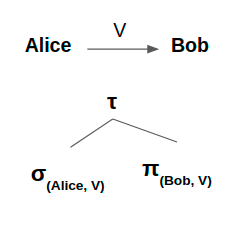
\includegraphics[width=0.3\columnwidth,keepaspectratio]{figures/utxo_growth/simplest_tx.png}
    \caption{The simplest expression of a transaction.}
    \label{fig:simplest_tx}
\end{figure}

Moving one step further, we assume three transactions $\tx_1$, $\tx_2$ and
$\tx_3$. The execution of these transactions is \emph{totally ordered}, \ie
$\tx_1 \rightarrow \tx_2 \rightarrow \tx_3$. Figure~\ref{fig:tx_order} depicts
this expression. Here, $\tx_1$ is nested within $\tx_2$ and both are nested
within $\tx_3$. Such tree is executed from bottom to top, therefore $\tx_2$ is
given the ledger state generated after $\tx_1$ is executed; similarly, $\tx_3$
is given the ledger state generated after both $\tx_1$ and $\tx_2$ are
executed. Given the above, we next define \emph{subtransactions};
interestingly, transactions may spend outputs created from their
subtransactions, thus we also define the notion of \emph{correlated
transactions}.

\begin{figure}[h!]
    \centering
    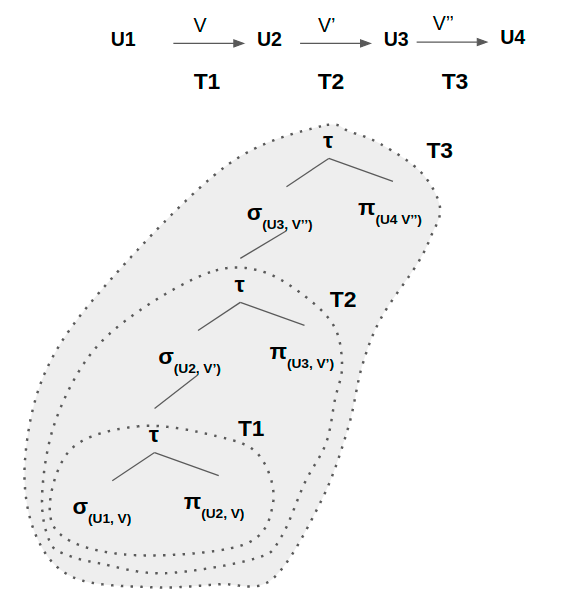
\includegraphics[width=0.5\columnwidth,keepaspectratio]{figures/utxo_growth/tx_order.png}
    \caption{The expression tree entails a transaction execution total
            order.}
    \label{fig:tx_order}
\end{figure}

\begin{definition} \label{def:subtransaction}
    A \emph{subtransaction} is a transaction nested within a ``parent''
    transaction; it is executed first, so its impact on the ledger state is
    visible to the parent.
\end{definition}

\begin{definition} \label{def:correlated_tx}
    Two transactions $\tx_1, \tx_2$ are correlated, if $\tx_1$ is a
    subtransaction of $\tx_2$ and $\tx_2$ spends at least one output created by
    $\tx_1$.
\end{definition}
